\documentclass{article}
\usepackage[final]{nips_2018}
\usepackage[utf8]{inputenc}
\usepackage[T1]{fontenc}

\usepackage{hyperref}
\usepackage{url}
\usepackage{booktabs}
\usepackage{amsfonts}
\usepackage{nicefrac}
\usepackage{enumerate}
\usepackage{microtype}
\usepackage{graphicx}
\usepackage{amsmath}
\usepackage{amsthm}
\usepackage{caption}
\usepackage{multirow}
\usepackage{enumitem}
\usepackage{listings}
\usepackage{todonotes}

\renewcommand{\thesubsubsection}{\thesubsection\,\alph{subsubsection})}
\newcommand{\del}[2]{\ensuremath{\frac{\partial #1}{\partial #2}}}
\newcommand{\Ell}{\ensuremath{\mathcal{L}}}
\lstset{basicstyle=\ttfamily\footnotesize,breaklines=true}

\title{Assignment 2\\Recurrent Neural Networks and Graph Neural Networks}

\author{
  Francesco Dal Canton \\
  \texttt{f.dal.canton@student.uva.nl} \\
  12404225
}

\begin{document}

\maketitle

%################################# NEW SECTION ##################################
\section{Vanilla RNN versus LSTM}

%###################### NEW SUBSECTION #######################
\subsection{Toy Problem: Palindrome Numbers}

%###################### NEW SUBSECTION #######################
\subsection{Vanilla RNN in PyTorch}

\begin{enumerate}[label=\textbf{1.\arabic*}]
  \item
  Throughout this assignment I use the notation $x_T$ in place of $x^{(T)}$ used in the assignment text. I also make the choice to ignore the $tanh$ function, which would only appear as an additional $\partial$-term in each application of the chain rule.

  That said, we can easily write the expression for the gradient of the loss w.r.t. the output weights as follows.

  \begin{align*}
    \del{\Ell_T}{W_{ph}} &= \del{\Ell_T}{\hat{y}_T} \del{\hat{y}_T}{p_T} \del{p_T}{W_{ph}} \\
    &= \del{\Ell_T}{\hat{y}_T} \del{\hat{y}_T}{p_T} h_T^T
  \end{align*}

  Defining the gradient w.r.t the hidden weights is trickier. We can start by writing out the standard chain rule formulation, which we can compress by omitting parts that we've defined in the previous assignment (i.e. cross-entropy, softmax, etc.).

  \begin{align*}
    \del{\Ell_T}{W_{hh}} &= \del{\Ell_T}{\hat{y}_T} \del{\hat{y}_T}{p_T} \del{p_T}{h_T} \del{h_T}{W_{hh}} \\
    &= \del{\Ell_T}{h_T} \del{h_T}{W_{hh}}
  \end{align*}

  We notice that any $h_t$ depends recursively on $h_{t-1}$ which itself depends on $W_{hh}$. We can then define the gradient of the last hidden state w.r.t. its weights, and develop it using the product rule.

  \begin{align*}
    \del{h_T}{W_{hh}} &= \del{\left[ W_{hx} x_T + W_{hh} h_{T-1} + b_h \right]}{W_{hh}} \\
    &= \del{\left[ W_{hh} h_{T-1} \right]}{W_{hh}} \\
    &= \del{W_{hh}}{W_{hh}} h_{T-1} + W_{hh} \del{h_{T-1}}{W_{hh}} \\
    &= h_{T-1} + W_{hh} \del{h_{T-1}}{W_{hh}}
  \end{align*}

  Where, at the end of the recursive chain, we reach the gradient of $h_0$ w.r.t. the hidden weights, which is $0$. With this knowledge, we can expand the chain in order to compress it again.

  \begin{align*}
    \del{h_T}{W_{hh}} &= h_{T-1} + W_{hh} \left( h_{T-2} + W_{hh} \left( h_{T-3} + W_{hh} \left( \dots \right) \right) \right) \\
    &= h_{T-1} + W_{hh} h_{T-2} + W_{hh}^2 h_{T-3} + \dots + W_{hh}^{T-2} h_{T-(T-1)} \\
    &= \sum_{i=1}^{T-1} W_{hh}^{i-1} h_{T-i}
  \end{align*}

  So that we can express the original gradient as:

  \begin{align*}
    \del{\Ell_T}{W_{hh}} &= \del{\Ell_T}{h_T} \sum_{i=1}^{T-1} W_{hh}^{i-1} h_{T-i}
  \end{align*}

  The most striking difference between the gradient of the loss w.r.t. the output weights and the one w.r.t. the hidden weights is that the latter involves a temporal dependency that extends all the way to the first time step of the cell's operation. In other words, after feeding the RNN a sequence of $n$ inputs, in order to perform backpropagation we need to multiply the gradient by the hidden weight matrix a large number of times, which grows exponentially with the number of time steps.

  This fact causes the well known problem of vanishing or exploding gradients. When performing an update over a large number of timesteps, the gradient that should pertain to the gradients further back in time either reduces to $0$ or it increases to infinity, depending on whether the hidden weights are small or large. This makes it very hard to train such networks for long sequences, since those longer time dependencies can't be learned.

  \item
  The implementation of the vanilla recurrent neural network was done as instructed.

  In the \texttt{train.py} script, this line of code is used:
  \begin{lstlisting}[language=Python]
  torch.nn.utils.clip_grad_norm_(model.parameters(),
                                 max_norm=config.max_norm)
  \end{lstlisting}
  Note that \texttt{clip\_grad\_norm\_} was used instead of \texttt{clip\_grad\_norm} since the latter is deprecated. This is a way to avoid the problem of exploding gradients. This function clips the maximum value of the norm of the gradients. The effect is that there is no risk of multiplying gradients of high magnitude over and over, thus leading to huge update steps that make it impossible for the network to learn. Note, however, that the vanishing gradient problem still exists since the gradients can have a very low norm.

  \item\label{q:vanilla_exp}
  After the first rounds of experimentation, I noticed sudden drops in training accuracy after convergence, which all quickly recovered. I attribute those to the exploding gradients, and tried using lower values for the maximum norm value used in the clipping of the gradients. After trying values of $10$, $5$, $2$, $1$, and $0.5$ with a baseline sequence length of 5, however, I realised that except for slight variations the problem still occurred. As such I decided to stick with the original value of $10$. All other parameters were kept at their default values.

  The strategy used to detect convergence is as follows: each $200$ training steps, the average accuracy is computed for the last $200$ steps. When the absolute difference between the current average accuracy and the previous average accuracy is smaller than $10^{-4}$, we say that the model has converged, and store the last average accuracy. The tested input lengths were in the range $[5, 35]$. The result is shown in Figure \ref{fig:results_vanilla}.

  \begin{figure}[ht]
      \centering
      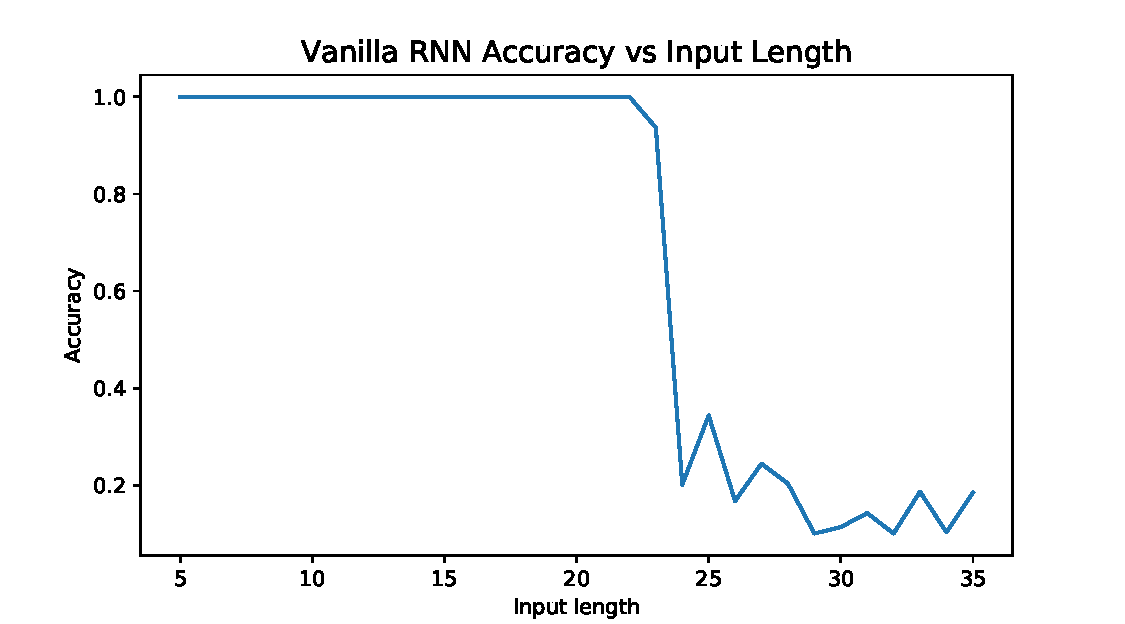
\includegraphics[scale=0.6]{img/results_vanilla.pdf}
      \caption{Average accuracy of the Vanilla RNN model in the last 200 training steps plotted against input length.}
      \label{fig:results_vanilla}
  \end{figure}

  \item
  The advantage of RMSprop is the usage of an adaptive learning rate. This element comes into play as the parameter update is calculated using a running average of the previous squared gradients, weighted according to the decay hyper-parameter. The result is that each new gradient is normalized based on the norms of the current and previous gradients. This leads to a sensible way of reducing the damage caused by exploding gradients.

  Adam works in a similar way, but it also incorporates a momentum term. This is done by computing the next gradient update as a running weighted average of the previous gradients, each of which is normalized in a way similar to that which RMSprop uses. The effect is that each parameter update is influenced by the gradients that preceded it: if the gradient is descending a steep hill it will accelerate, while if it is traversing a mostly flat region with uncertain topology it will slow down.

  Both of these strategies are beneficial towards training, and they surpass SGD in training speed and accuracy.
\end{enumerate}

%###################### NEW SUBSECTION #######################
\subsection{Long-Short Term Network (LSTM) in PyTorch}

\begin{enumerate}[label=\textbf{1.\arabic*}]
  \setcounter{enumi}{4}
  \item
  \begin{enumerate}[label=\textbf{(\alph*)}]
    \item
    The input modulation gate $\mathbf{g}^{(t)}$ determines how each feature of the input affects the hidden state of the LSTM cell given the previous hidden state. Since the nonlinearity used in this gate is the $tanh$ function, each output feature will be in the range $(-1, 1)$, which makes sense since it normalizes the effect that each variable may have on the cell state, while also centering the activations around $0$.

    The input gate $\mathbf{i}^{(t)}$ determines how much influence each feature update, computed using $\mathbf{g}^{(t)}$, should affect the cell state. The softmax nonlinearity is a good choice for this purpose since its value is in the range $(0, 1)$. This means that when $\mathbf{i}^{(t)}$ is multiplied with $\mathbf{g}^{(t)}$, the magnitude of each feature update is modulated, but it can never exceed the original range of $(-1, 1)$.

    The forget gate $\mathbf{f}^{(t)}$ is similar in nature to the input gate: it modulates the magnitude of the cell state as it flows through the cell, thus controlling which features are forgotten and which ones are left unchanged. The nonlinearity used in this gate is again the softmax function. For the same reason as the input gate, multiplying each feature of the cell state with a number in the range $(0, 1)$ makes it so that each feature is reduced in magnitude if it should be forgotten, and left unchanged if not (with all the steps inbetween).

    The output gate $\mathbf{o}^{(t)}$ works once again in a similar way: it controls which parts of the cell state are forgotten, so that the rest is both given as the cell output and as the hidden state for the next time step. This gate works with the well chosen sigmoid nonlinearity according to the same principle as described in the previous two paragraphs. The cell state, after being passed through a $tanh$ function, is filtered by modulating the magnitude of each filter.

    \item
    In calculating the number of trainable parameters, both $T$ and $m$ don't come into play, since the parameters are shared across time steps and batch samples. To compute the number of parameters, it suffices to sum the number of parameters of each weight matrix used on the input ($n \times d$), of each weight matrix used on the hidden and cell states ($n \times n$), and of each bias vector ($n$). The result is:

    \begin{align*}
      N &= 4 (n \times d) + 5 (n \times n) + 5 n \\
      &= 5n^2 + 9n + 4d
    \end{align*}

  \end{enumerate}

  \item
  The LSTM network was implemented as instructed. The only difference was, instead of summing the linear transformations of input and previous hidden state, the two were concatenated and linearly transformed with a combined weight matrix.

  The experimental setup for evaluating this model was identical to that used in question \ref{q:vanilla_exp}. The results are shown in Figure \ref{fig:results_lstm}.

  \begin{figure}[ht]
      \centering
      \includegraphics[scale=0.6]{img/results_LSTM.pdf}
      \caption{Average accuracy of the LSTM model in the last 200 training steps plotted against input length.}
      \label{fig:results_lstm}
  \end{figure}

  The main difference between the performance of the Vanilla RNN and the LSTM is the input length which first becomes difficult for the model to deal with: 24 for the former, and 34 for the latter. It is worth noting, when looking at the LSTM plot, that in previous runs of the experiment the decrease in performance occurred sometimes for shorter sequences and sometimes for longer ones. However on average the LSTM is still able to learn longer sequences compared to the Vanilla RNN. This has to do with two main factors, both related to the ingenious design of the LSTM's gates.

  The first factor is related to the function used to compute the next cell state $\mathbf{c}^{(t)}$. Since this occurs with an addition, the gradient which comes into play when backpropagating through time will have a value of $1$, thus reducing problems related to the vanishing or exploding gradient. This due to the fact that $1^n = 1$.

  The second factor has to do with the flow of information inside of the LSTM cell: the input modulation gate, the input gate, the forget gate, and the output gate all serve the purpose of filtering information that flows through the cell, so as to maximise the flow of information useful for the task, and minimise the flow of useless information or noise. This has the effect of saturating and polluting the cell's state much more slowly, thus allowing for longer retention of useful information.
\end{enumerate}

%################################# NEW SECTION ##################################
\section{Recurrent Nets as Generative Model}

\begin{enumerate}[label=\textbf{2.\arabic*}]
  \item

  \begin{enumerate}[label=\textbf{(\alph*)}]
    \item
    The model was implemented and trained as instructed. A dropout rate of $0.2$ was used, along with a learning rate decay of $0.96$ every $5\,000$ steps. All other parameters were set to default. The model's performance plateaud around an accuracy of $0.1$ and a loss of $1.2$, and was trained for $50\,000$ steps on two novels by Alexandre Dumas. While low, the low accuracy seems reasonable for two reasons. The first is that the dataset itself is around $2.5$ million characters long, with a vocabulary size of $81$. This means that, in $50\,000$ steps, the whole dataset is seen only one and a half times. This is not enough to memorise any full sequence of words, and the model rather learns a generalised pattern. The other issue is that the english language uses many short words, in such a way that given one word it will be very hard to accurately predict which word follows: for instance, the verb `stand' may be followed by `up' just as likely as `down' or `still'. This makes sentences often unpredictable.

    \item
    Here I report five sentences of length $T = 30$ obtained at evenly spaced intervals during training: starting at step $0$ every $1\,000$ steps.
    \begin{lstlisting}
  [0] :In'])G*T-Ms9F
  VgKrTlmlha5p7!y

  [1000]  to me to ke elouthreated pall

  [2000] for ihune in not plEand back t

  [3000] an which! d'Artagnan.
  EI.
  If t

  [4000]  of Madame de Treville. "I nev
    \end{lstlisting}

    The progress of the LSTM's training is clear. In the first example, we see a completely random sequence of characters, with no apparent pattern.

    The second example shows a twofold improvement. The characters now come from a specific subset, which is that of lowercase letters, the most common type of characters in the dataset. Along with lowercase letters, spaces are now distributed in a reasonable way: the words have a reasonable length. Additionally, small very common words such as `to' and `me' appear in the sentence.

    The third example shows a slight improvement over the previous, and slightly longer words appear, such as `for' and `back'.

    By the fourth example not all words are real, but some common longer words have been learned: `d'Artagnan' is the name of the main character in the two training novels, so it has been learned despite its length.

    Finally, by the last example most words have been learned, and some of the outputs are written in good English. In this case, the whole sentence could very well be a small extract from a sentence, with accurate punctuation.

    \item
    The temperature parameter $T$ was included by computing the sampling probability $\textbf{p}_T$ as:

    \begin{align*}
      \textbf{p}_T &= \sigma\left( \frac{\textbf{p}}{T} \right)
    \end{align*}

    Where $\sigma$ is the softmax function.

    Here I report two sentences per temperature setting.
    \begin{lstlisting}
  [ 0.5 ] e as a specious and things of
  [ 0.5 ] enting the pieces of the great
  [ 1.0 ] than for him, in order
  that gr
  [ 1.0 ]  CALLET
  Fortunity, it murmured
  [ 2.0 ] Amenutny! Onage!"

  Muria, knel
  [ 2.0 ] O2N THEEINFOU;-Cord? Nothing c
    \end{lstlisting}

    We know, looking at the formula, that a low temperature will yield a more peaked sampling probability distribution, meaning that the model's best guess' probability will tend towards $1$. This is reflected in the sentences produced with $T = 0.5$, which contain mostly well-formed english words, or at least believable ones. As the temperature increases to $1.0$ which is the standard sampling strategy, the sentences still seem believable but there are slight inconsistencies, which happen for instance as semi-random newlines. At $2.0$, the sentences look very strange, as some words are real while others seem like inconsistent sequences of common characters. This makes sense as the sampling strategy is tending more towards uniform sampling.
  \end{enumerate}

  \item
  Here I include three sentences produced with a temperature of $0.7$ and $T = 60$. Note that the newlines in the first and third example were inserted manually to avoid the lines extending over the page's margins.

  \begin{verbatim}
  [Start] The boy
  [Model says] The boy and the sentiments of the end of the street
  and still so muc

  [Start] Athos decided
  [Model says] Athos decided the door of the staircase.

  “Well,” said Manicamp, “the devi

  [Start] Madam
  [Model says] Madame, and said to her eyes from his hand to the four
  friends to
  \end{verbatim}

  The outputs show that, while the model is able to form coherent words and semi-coherent sentences, it struggles with long term dependencies and broad syntactical structures. This is reasonable since it was trained on short text fragments that can't contain such long structures.
\end{enumerate}

%################################# NEW SECTION ##################################
\section{Graph Neural Networks}

%###################### NEW SUBSECTION #######################
\subsection{GCN Forward Layer}

\begin{enumerate}[label=\textbf{3.\arabic*}]
  \item

  \begin{enumerate}[label=\textbf{(\alph*)}]
    \item
    The structural information in the GCN layer is used via the multiplication with matrix $\hat{A}$. This matrix contains the normalized graph structure, which means that it captures the connections between nodes in the graph, allowing for the propagation of information between neighboring nodes. This way, the information so far propagated to each node is further propagated to that node's neighbors, performing what could be described as message passing.

    \item
    Since each layer propagates information through one `hop' or neighborhood, covering three hops would require three layers.
  \end{enumerate}
\end{enumerate}

%###################### NEW SUBSECTION #######################
\subsection{Applications of GNNs}

\begin{enumerate}[label=\textbf{3.\arabic*}]
  \setcounter{enumi}{1}
  \item
  In \cite{segmentation} Graph Neural Networks are used for pixel segmentation in computer vision. Using k-nearest neighbors, a graph is produced where nodes correspond to sets of pixels in the image. The graph is then used as input to a GNN to produce pixel-level representations used then for semantic segmentation.

  \cite{molecular} shows an approach for molecular fingerprinting which uses GCNs on the graph structure of molecules to generate useful representations of said molecules, which are then used in a variety of tasks.

  Another interesting application is shown in \cite{relational}, which reports state-of-the-art results in text-based question answering using relation networks, thus operating on text and images. This application is remarkable in that it operates on knowledge graphs, and it allows for improved performance on general reasoning tasks by including relational information.
\end{enumerate}

%###################### NEW SUBSECTION #######################
\subsection{Comparing and Combining GNNs and RNNs}

\begin{enumerate}[label=\textbf{3.\arabic*}]
  \setcounter{enumi}{2}
  \item

  \begin{enumerate}[label=\textbf{(\alph*)}]
    \item
    The first thing to realize is that the two types of networks work best with two similar but distinct types of data. RNNs such as LSTMs work best with sequential data, where there exist dependencies and interactions across the sequence's single dimension. On the other hand, GNNs such as CGNs work best with graph data, meaning that the sequences under consideration may split, and contain cyclical relations.

    Choosing RNNs over GNNs for a certain task might be a good choice when there is no graph data available for a certain task, while GNNs might be more of a general choice for when this data is available.

    As an example, consider the task of sentence or paragraph representation. An LSTM might be a good choice for such a task, since text is sequential and, in the absence of more information, its relational dependencies flow forward in the sequence. In other words, textual elements normally depend on what came before, and rarely on what comes after. RNNs are able to encapsulate the forward propagating infromation and use it to contextualize each new word or character's impact on the representation.

    On the other hand, if we have information about the tree structure of the text that we are using, performing the same task using some GNN-based architecture might yield better results. The GNN will be able to capture relations within the text which are not only forward flowing, but also backward flowing. By using the tree structure of a sentence, the hierarchical position of each word in the syntactic tree would allow for top-down and bottom-up influences between different hierarchical levels of the tree. This might allow for more detailed and accurate representations of sentences.

    \item
    RNNs and GNNs could be used in a combined model to produce a generalized version of GCNs. In its basic definition, such a model could be defined as:

    \begin{align*}
      H^{(t+1)} &= f\left( \hat{A} H^{(t)} W \right)
    \end{align*}

    Where the weight matrix $W$ is shared across all cells of the network. This could be applied on any task that GCN is already applied to, and it would allow for a propagation across an arbitrary number of neighborhoods depending on the time-steps that are performed. Unfortunately, this type of network would still be highly susceptible to the vanishing and exploding gradient problems.
  \end{enumerate}
\end{enumerate}

\bibliography{bibliography}
\bibliographystyle{unsrt}

\end{document}
